\documentclass{article}
\usepackage[spanish]{babel}
\usepackage[utf8x]{inputenc}
\usepackage{graphicx}
\usepackage{subfigure}
\usepackage{hyperref}
\usepackage{amssymb}
\usepackage{textcomp}
\usepackage{booktabs}
\usepackage[inline]{enumitem}
\hypersetup{colorlinks=true,citecolor=black,filecolor=black,linkcolor=black,urlcolor=black}
\usepackage{amsmath}
\usepackage{amsfonts}

\usepackage{algorithm}
\usepackage{algorithmic}
\floatname{algorithm}{Algoritmo}
\renewcommand{\listalgorithmname}{Lista de algoritmos}
\renewcommand{\algorithmicrequire}{\textbf{Entrada:}}
\renewcommand{\algorithmicensure}{\textbf{Salida:}}
\renewcommand{\algorithmicend}{\textbf{fin}}
\renewcommand{\algorithmicif}{\textbf{si}}
\renewcommand{\algorithmicthen}{\textbf{entonces}}
\renewcommand{\algorithmicelse}{\textbf{si no}}
\renewcommand{\algorithmicelsif}{\algorithmicelse,\ \algorithmicif}
\renewcommand{\algorithmicendif}{\algorithmicend\ \algorithmicif}
\renewcommand{\algorithmicfor}{\textbf{para}}
\renewcommand{\algorithmicforall}{\textbf{para todo}}
\renewcommand{\algorithmicdo}{\textbf{hacer}}
\renewcommand{\algorithmicendfor}{\algorithmicend\ \algorithmicfor}
\renewcommand{\algorithmicwhile}{\textbf{mientras}}
\renewcommand{\algorithmicendwhile}{\algorithmicend\ \algorithmicwhile}
\renewcommand{\algorithmicloop}{\textbf{repetir}}
\renewcommand{\algorithmicendloop}{\algorithmicend\ \algorithmicloop}
\renewcommand{\algorithmicrepeat}{\textbf{repetir}}
\renewcommand{\algorithmicuntil}{\textbf{hasta que}}
\renewcommand{\algorithmicprint}{\textbf{imprimir}} 
\renewcommand{\algorithmicreturn}{\textbf{devolver}} 
\renewcommand{\algorithmictrue}{\textbf{cierto }} 
\renewcommand{\algorithmicfalse}{\textbf{falso }} 

\usepackage{blindtext}

\begin{document}
\title{
	\begin{figure}[!ht]
	\centering
		
\includegraphics[scale=0.8]{../resources/cinvestav-logo}
		\\[0.5cm]LTI Cinvestav Tamaulipas
	\end{figure}
	\vspace{1cm}
	Inteligencia de enjambre (Swarm Intelligence) -\\ Optimización por cúmulo de partículas (Particle Swarm Optimization PSO){\small[2.b.i-iii]}
	\vspace{1cm}
}
	
\author{Rafael Pérez Torres}	
		
\date{
	Tópicos Selectos en Reconocimiento de Patrones \\ 
	\vspace{0.8cm}
	Profesor Dr. Wilfrido Gómez Flores \\
	\vspace{1cm}
	%\today
}

\maketitle
% \setlength{\parindent}{0pt}

\begin{abstract}
Este documento presenta una breve introducción a la inteligencia computacional, haciendo énfasis en las metodologías de inteligencia de enjambre como técnicas de optimización para la resolución de problemas.
En particular, se describe el algoritmo de Optimización por Cúmulo de Partículas (PSO, Particle Swarm Optimization), así como un conjunto de sus variantes.
\end{abstract}

\section{Introducción}
La mayor motivación para el desarrollo de la algoritmia es el diseño de modelos algorítmicos para solucionar problemas de alta complejidad.
Muchos beneficios han sido obtenidos a través de la construcción de modelos basados en inteligencia natural y biológica, obteniendo los llamados \emph{sistemas inteligentes}.
En conjunto con lógica, razonamiento deductivo, sistemas expertos, razonamiento basado en casos y sistemas de aprendizaje máquina simbólicos, los algoritmos inteligentes forman parte del área de inteligencia artificial.
De acuerdo a la junta de redes neuronales de la IEEE celebrada en 1996, la inteligencia artificial se define como el estudio de cómo hacer que las computadoras hagan cosas en las que la gente (todavía?) es mejor.


La inteligencia computacional es a su vez, el estudio de mecanismos adaptativos que habiliten o faciliten el comportamiento inteligente en entornos altamente cambiantes y complejos.
Estos mecanismos incluyen a los paradigmas de la IA que exhiben una habilidad para aprender o adaptarse a nuevas situaciones, a generalizar, abstraer, descubrir y asociar.
Dentro de la inteligencia computacional se encuentran los siguientes paradigmas, ilustrados en la Figura~\ref{fig:paradigmas-inteligencia-computacional}:
\begin{itemize}
	\item Redes neuronales artificiales (NN, Neural Networks)
	\item Cómputo evolutivo (EC, Evolutive Computing)
	\item Inteligencia de enjambre (SI, Swarm Intelligence)
	\item Sistemas inmunes artificiales (AIS, Artificial Immune Systems)
	\item Sistemas difusos (FS, Fuzzy Systems)
\end{itemize}

\begin{figure}[tb]
	\centering
	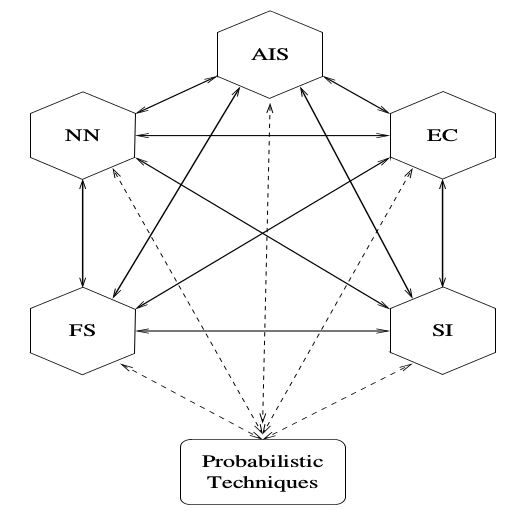
\includegraphics[scale=0.25]{../resources/paradigmas-inteligencia-computacional}
	\caption{Los algoritmos inteligentes o paradigmas de la inteligencia computacional}
	\label{fig:paradigmas-inteligencia-computacional}
\end{figure}
Mientras que las distintas técnicas de estos paradigmas han sido aplicados de forma exitosa para solucionar problemas del mundo real, la tendencia actual consiste en desarrollar hibridaciones de estos paradigmas debido a que ninguno es superior a los demás en todos los escenarios.
De esta forma, se permite rescatar y enfocarse en las fortalezas de los componentes de un sistema híbrido, eliminando sus debilidades.

Cada uno de los paradigmas previamente mencionados ha tenido su origen en sistemas biológicos.
Las redes neuronales modelan sistemas neurológicos presentes en los seres vivos, el cómputo evolutivo modela la evolución natural (incluyendo evolución genética y de comportamiento), la inteligencia de enjambre modela el comportamiento social de organismos viviendo en enjambres o colonias, los sistemas inmunes artificiales modelan el sistema inmune humano, y lós sistemas difusos se originaron a partir de los estudios de cómo los organismos interactúan con su entorno.

\section{Introducción a la inteligencia de enjambre}
Supongamos que un grupo de amigos busca un tesoro y conocen aproximadamente dónde se encuentra.
Los integrantes del grupo acuerdan un mecanismo para compartir el tesoro de modo que todos los que participan sean recompensados, pero la persona que lo encuentra tenga una recompensa mayor y que el resto de los integrantes reciba una recompensa proporcional a la distancia a la que se encontraban cuando el tesoro fue descubierto.
Supóngase además que cada integrante tiene un detector de metal y puede comunicar la intensidad de la señal y su ubicación a sus vecinos más cercanos.
De esta forma, cada persona sabe si alguno de sus vecinos está más cerca del tesoro que ella misma.
Al saberlo, se pueden tomar dos acciones:
\begin{itemize}
	\item Ignorar a los amigos, si una persona lo encuentra será por completo para ella, pero si no lo encuentra se queda con las manos vacías.
	\item Utilizar la información de los vecinos y moverse en la dirección del amigo más cercano con la señal más intensa (el que está más cerca del tesoro).
	Al utilizar la información local, se incrementan las posibilidades de encontrar el tesoro, o al menos de maximizar la recompensa.
\end{itemize}

El anterior es un ejemplo extremadamente simple de los beneficios de la cooperación en situaciones donde un sólo integrante no tiene el conocimiento total o global del entorno.
Los individuos del grupo interactúan entonces para solucionar el objetivo global al intercambiar información disponible localmente, lo cual al final se propaga a todo el grupo de tal forma que el problema se resuelve de forma más eficiente que lo que podría realizar un individuo.
En términos muy amplios, el grupo puede ser considerado un \textbf{enjambre}.
Formalmente, un enjambre puede ser definido como u\emph{n grupo de agentes (generalmente móviles) que se comunican entre ellos para actuar en su entorno local}.
Las interacciones entre agentes resultan en estrategias colectivas de solución de problemas distribuídas.

La inteligencia de enjambre se refiere al comportamiento que permite solucionar problemas y que emerge de la interacción entre dichos agentes, y la inteligencia computacional de enjambre se refiere a modelar algorítmicamente este comportamiento.
Formalmente, la inteligencia de enjambre \emph{es la propiedad de un sistema que permite que a partir del comportamiento colectivo de agentes simples que interactúan localmente con su entorno, emerjan patrones globales de funcionamiento coherente}.
La inteligencia de enjambre ha sido también denominada como \emph{inteligencia colectiva}.
Swarm intelligence has also been referred to as collective intelligence.




\section{Optimización por cúmulo de partículas}
Swarm intelligence (SI) originated from the study of colonies, or swarms of social or-
ganisms. Studies of the social behavior of organisms (individuals) in swarms prompted
the design of very efficient optimization and clustering algorithms. For example, sim-
ulation studies of the graceful, but unpredictable, choreography of bird flocks led to
the design of the particle swarm optimization algorithm, and studies of the foraging
behavior of ants resulted in ant colony optimization algorithms.

\subsection{Algoritmo PSO básico}
Particle swarm optimization (PSO) is a stochastic optimization approach, modeled on
the social behavior of bird flocks. PSO is a population-based search procedure where
the individuals, referred to as particles, are grouped into a swarm. Each particle in
the swarm represents a candidate solution to the optimization problem. In a PSO
system, each particle is “flown” through the multidimensional search space, adjusting
its position in search space according to its own experience and that of neighboring
particles. A particle therefore makes use of the best position encountered by itself
and the best position of its neighbors to position itself toward an optimum solution.
The effect is that particles “fly” toward an optimum, while still searching a wide area
around the current best solution. The performance of each particle (i.e. the “closeness”
of a particle to the global minimum) is measured according to a predefined fitness
function which is related to the problem being solved. Applications of PSO include
function approximation, clustering, optimization of mechanical structures, and solving
systems of equations.
Studies of ant colonies have contributed in abundance to the set of intelligent algo-
rithms. The modeling of pheromone depositing by ants in their search for the shortest
paths to food sources resulted in the development of shortest path optimization al-
gorithms. Other applications of ant colony optimization include routing optimization
in telecommunications networks, graph coloring, scheduling and solving the quadratic
assignment problem. Studies of the nest building of ants and bees resulted in the
development of clustering and structural optimization algorithms.

Individuals in a particle swarm follow a very simple behavior: to emulate the success of
neighboring individuals and their own successes. The collective behavior that emerges
from this simple behavior is that of discovering optimal regions of a high dimensional
search space.
A PSO algorithm maintains a swarm of particles, where each particle represents a
potential solution. In analogy with evolutionary computation paradigms, a swarm is similar to a population, while a particle is similar to an individual. In simple terms,
the particles are “flown” through a multidimensional search space, where the position
of each particle is adjusted according to its own experience and that of its neighbors.
Let x i (t) denote the position of particle i in the search space at time step t; unless
otherwise stated, t denotes discrete time steps. The position of the particle is changed
by adding a velocity, v i (t), to the current position, i.e. ...


Las condiciones de paro están en Engelbert
PSO no garantiza la obtención de una solución optimal en todos los casos.
\subsection{Variantes de PSO}
PSO binaria, discreta y combinatoria

Como las ecuaciones usadas en PSO operan con números reales, un método común a la hora de resolver problemas discretos es mapear el espacio de búsqueda a un dominio continuo, para aplicar PSO clásica, y luego desmapear el resultado. El proceso de mapeo puede consistir en una conversión muy simple (por ej. redondeo de valores) o, por el contrario, bastante compleja.45

Sin embargo, las ecuaciones de movimiento hacen uso de operadores que controlan cuatro acciones:

    calcular la diferencia entre dos posiciones (el resultado define un desplazamiento)
    multiplicar una velocidad por un coeficiente numérico
    sumar dos velocidades
    aplicar una velocidad a una posición

Generalmente, la posición y la velocidad están representadas por n números reales, y los operadores básicos son -, *, +. Pero tales entidades matemáticas pueden definirse de una manera completamente diferente, a fin de hacer frente a problemas binarios (o discretos, en un sentido más amplio), e incluso combinatorios.46 47 48 .49 Una estrategia es redefinir los operadores como basados en conjuntos.50
(Wikipedia)
\blindtext[3]
\subsection{Vecindarios y topologías}
\blindtext[3]


\nocite{*}
\bibliographystyle{plain}
\bibliography{references} 

\end{document}